\subsection{Experiment 1: Using Symbols to Improve the Effectiveness of Learning} \label{sec:experiment-1}

\subsubsection{Objective}

The goal of this experiment is to demonstrate the validity of our hypothesis by showing that the presence of a clear and concise symbolic representation of the input data improves the learning accuracy of the models developed. The symbols are analogous to the shared knowledge used by human learners to overcome the difficulty in learning from a limited number of noisy examples as discussed in Section \ref{sec:theory-hypothesis}. This first experiment deals with models trained to perform addition only. Later experiments will expand the dataset to include all four basic arithmetic operations.

\subsubsection{Method}

We developed five models based on recurrent neural networks, specifically those based on LSTMs, that learn to sequentially add images of handwritten digits (see Figure \ref{fig:noisy-mnist}). When properly trained the network models can be queried with a sequence of two images, each representing a single digit, followed by an image of the ``+" operator.  The network will output two one-hot vectors representing the estimate of the sum of the input digits. One-hot vectors have all their features set to 0 except for the feature corresponding to the value being represented which is set to 1.

Alongside the handwritten digit input channel, the networks also have a second input channel meant to receive only a standard set of symbols. In the case of numeric digits, the symbols are of the digits zero through nine clearly rendered in a standard font. See Figure \ref{fig:symbols} for the symbolic images used in the experiment. After the five models are trained, the test set is applied to compare the effect of the two approaches of providing symbolic information, mentioned in Section \ref{sec:theory-approach-methodology-sequential-models}, on the accuracies of performing the addition, to the cases of having no symbolic data and only symbolic data.

As discussed in Section \ref{sec:theory-approach-the-mnist-dataset}, the MNIST dataset of handwritten digits is used to train and test all the models developed for all our experiments. A limited subset is sampled from the larger MNIST dataset to create an impoverished collection of examples that are used to train and test our models. The dataset is composed of two single digit inputs followed by the operator. For each of the 100 two digit combinations, we randomly sample ten examples from the MNIST database. For example, the 0 + 0 combination has 10 different examples sampled, the 0 + 1 combination has another 10 examples and so on. This number was chosen because it impoverishes the dataset and also provides room for improvement when introducing symbols. In total, one thousand different input/output pairs are composed. Figure \ref{fig:dataset-examples} shows example combinations, each combination having one sample from the MNIST dataset. Constructing the dataset in that way ensures that there is sufficient balance of training and testing examples for each combination.

\begin{figure}[t]
	\centering
	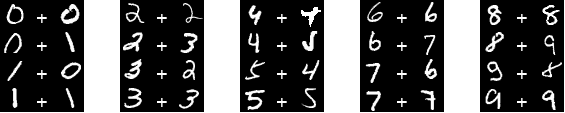
\includegraphics[max width=\textwidth]{dataset-examples}
	\caption{Some of the combinations of operands used for the experiment. Each combination shows only one sample selected from the MNIST dataset.}
	\label{fig:dataset-examples}
\end{figure}

A 5-fold cross-validation (discussed in Section \ref{sec:background-artificial-neural-networks-feed-forward-neural-networks}) approach is used to break down the dataset into a training, validation and test set such that for each combination of digits, six samples are used for training, two samples for validation and another two for testing. Since $k$ is set to 5, the training and testing of each of the five models is repeated five times, where the training, validation and testing samples for each combination are shuffled. The models for this experiment are exposed to all possible combinations of single digit operands during training. Some of the later experiments will only use a subset of the combinations for training and the rest for testing. After repeating the experiment five times for each model and recording the accuracies obtained from testing with the test sets, the mean accuracy and standard deviation for each model are calculated and used to compare the experiments graphically. A Hypothesis t-Test is also used to check the statistical difference of the means.

All networks trained have the same architecture, varying only in terms of the number of inputs. The architecture consists of two hidden LSTM layers, 512 units each, fully connected to an output layer, 20 units in length, composed of two one-hot vectors. This architecture was the result of trial and error and was found to have sufficient representation for the most difficult task at no detriment to the other tasks. The networks are trained using the Adam optimizer with the mean square error as the loss function and a learning rate of 0.001. Training is performed over 200 epochs (found to be sufficient for all methods) in batches of 100 and the set of weights performing best on the validation set is saved.  When evaluating the models, only noisy handwritten images are input and no symbol images are provided. The following paragraphs describe the five different architectures and training sets used.

\begin{figure}[t]
	\centering
	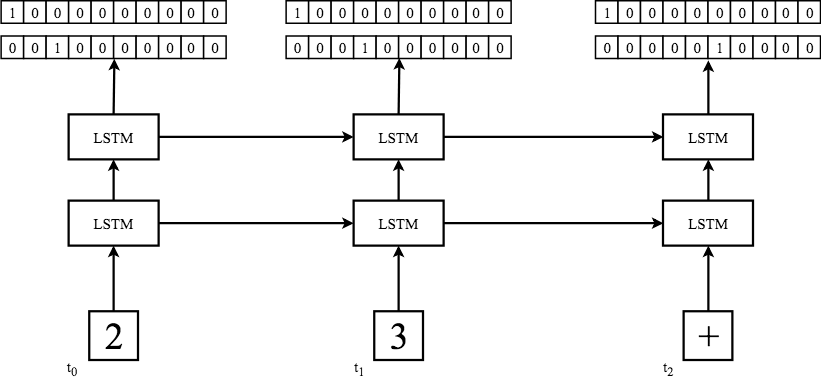
\includegraphics[max width=\textwidth]{sequential-model-symbols-only}
	\caption{Symbols Only (SO). A deep LSTM network that accepts a sequence of two operands and an operator. The operands are provided as the consistent symbol digits.}
	\label{fig:sequential-model-symbols-only}
\end{figure}

\paragraph{Symbols Only (SO).} The model learns to perform classification and addition using only the standard symbols (see Figure \ref{fig:sequential-model-symbols-only}). The input is a sequence of three 28x28 images, that are fed to the network one after the other. The first two images are that of the digits rendered clearly using a standard font. The third image is the plus operator. At each of the first two time steps the model is trained to classify the incoming digits producing two one-hot vectors representing the least and most significant digits of the input. Typically, the most significant digit will always be zero on these two time steps since we only use single digit inputs. When the plus sign is provided on the third time step, the network performs the addition operation, producing the result at the two one-hot vectors. The goal of training this model is to show that it is quite easy to do so using clear and consistent symbols.

\begin{figure}[t]
	\centering
	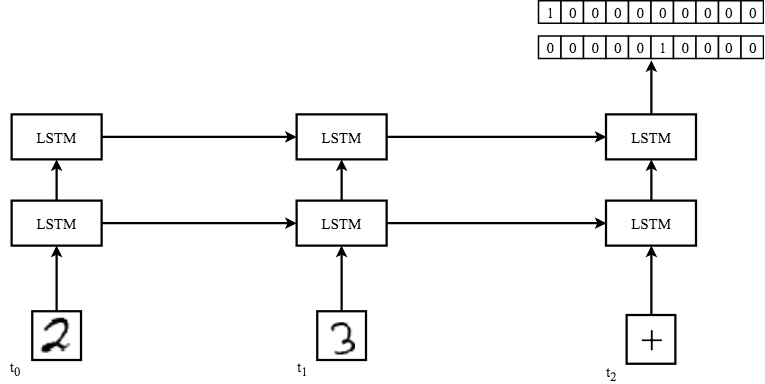
\includegraphics[max width=\textwidth]{sequential-model-noisy-only}
	\caption{Noisy Inputs Only (NO). A deep LSTM network that accepts a sequence of two operands and an operator. Only noisy operands are provided.}
	\label{fig:sequential-model-noisy-only}
\end{figure}

\paragraph{Noisy Inputs Only (NO).} The model learns to perform the addition using noisy handwritten digits without having to output the proper classes in the intermediate stages of the recurrent network (see Figure \ref{fig:sequential-model-noisy-only}). The input is a sequence of three 28x28 images, that are fed to the network one after the other. The first two images are that of noisy handwritten digit operands. The third image is the plus operator rendered in a standard font.  The goal of training the model using this method is to investigate the effectiveness of a network that is trained without the presence of symbols.

\begin{figure}[t]
	\centering
	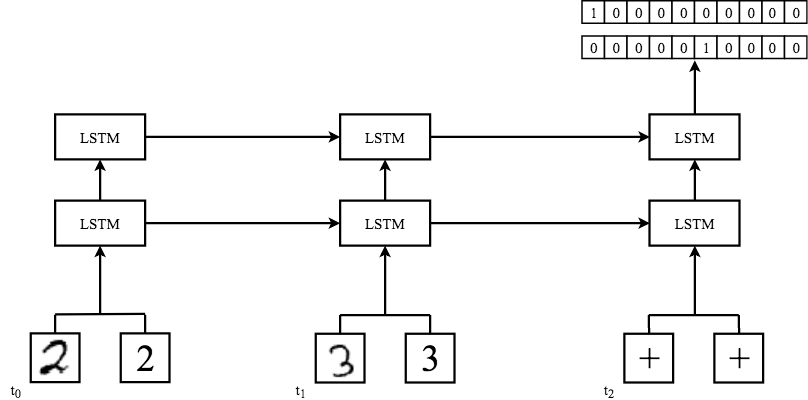
\includegraphics[max width=\textwidth]{sequential-model-symbols-noisy}
	\caption{Noisy and Symbol Inputs (NS). A deep LSTM network that accepts a sequence of two operands and an operator. Both the noisy operands and their corresponding symbolic information are provided alongside one another.}
	\label{fig:sequential-model-symbols-noisy}
\end{figure}

\paragraph{Noisy and Symbol Inputs (NS).} This model learns to perform addition without having to output the proper classes in the intermediate stages of the recurrent network (see Figure \ref{fig:sequential-model-symbols-noisy}). The input is a sequence of three pairs of 28x28 images, that are fed to the network one after the other. The first pair of images are of the first noisy handwritten digit operand and its matching standard symbolic digit. The second pair of images are for the second digit operand. The third pair of images are both the standard plus operator. The goal is to investigate the effect of introducing the clear symbol channel as an input (the explicit symbol) on the accuracy of the network.

\begin{figure}[t]
	\centering
	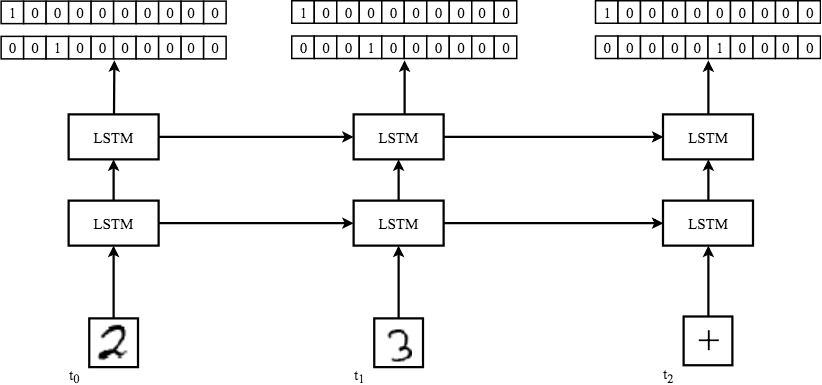
\includegraphics[max width=\textwidth]{sequential-model-noisy-classification}
	\caption{Noisy Inputs Only with Intermediate Classification (NC). A deep LSTM network that accepts a sequence of two operands and an operator. Noisy digits are provided as inputs and the network is trained to output the classes of each digit before performing the operation.}
	\label{fig:sequential-model-noisy-classification}
\end{figure}

\paragraph{Noisy Inputs Only with Intermediate Classification (NC).} The model learns to perform classification and addition on noisy digits only(see Figure \ref{fig:sequential-model-noisy-classification}). The input is a sequence of three 28x28 images, that are fed to the network one after the other. The first two images are that of handwritten digit operands. The third image is the plus operator. The model is trained to classify each incoming digit on each of the first two time steps by providing the class (as a one-hot vector) on the output during training and then perform the operation on the third time step. The goal is to investigate the effect of symbols on the accuracy of the network. However instead of using explicit symbols as inputs, the symbol is embedded in the LSTM context. By providing the classes of the handwritten digits while training, we believe that the network learns the symbolic information implicitly in the recurrent weights and then uses this information to aid in performing the mathematical operation.

\begin{figure}[t]
	\centering
	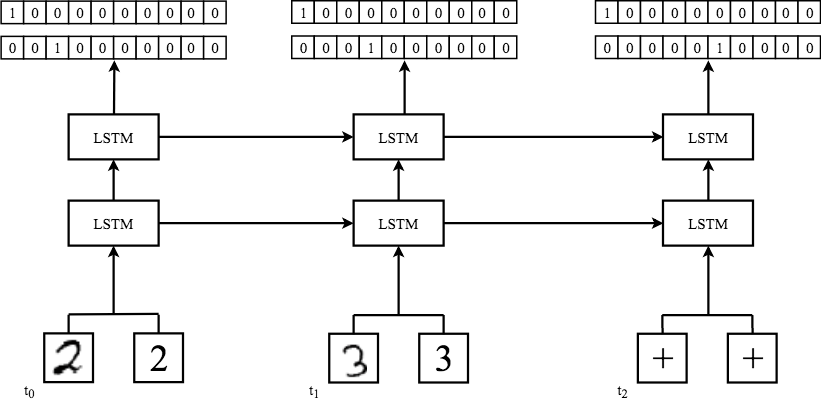
\includegraphics[max width=\textwidth]{sequential-model-noisy-symbol-classification}
	\caption{Noisy and Symbol Inputs with Intermediate Classification (NX). A deep LSTM network that accepts a sequence of two operands and an operator. Both the explicit and implicit symbols are provided.}
	\label{fig:sequential-model-noisy-symbol-classification}
\end{figure}

\paragraph{Noisy and Symbol Inputs with Intermediate Classification (NX).} This last model combines both methods of training used in NS and NC where the input includes the clear symbolic channel and the input classes are also provided on the output channel during training (see Figure \ref{fig:sequential-model-noisy-symbol-classification}). Here we investigate if a combination of the two methods of symbolic input improves on the individual approaches of the previous two methods.

\bigskip

While testing the trained Symbols Only (SO) model, we also test how well that model performs when tested on noisy handwritten digit inputs. We call this testing attempt \textbf{Symbols Tested with Noisy Inputs (SN)}. The objective is to see if training a recurrent neural network using only the idealized symbols will help the resulting model filter out the noise seen in the handwritten digits.

\subsubsection{Results}

\begin{table}[p!]
	\center
	\caption{A comparison of the mean accuracy and standard deviation of the models developed by the five methods. Also shown is the p-value of a hypothesis t-Test when compared to the NO method.}
	\label{tab:experiment-1-results-table}
	\begin{tabular}{ |c|c|c|c| } 
		\hline
		Method & Accuracy (\%) & Standard Deviation  & p-value, t-Test with NO Method\\ 
		SO & 100 & 0 & NA\\ 
		SN & 32.73 & 6.9 & NA\\
		NO & 60.16 & 4.5 & NA \\ 
		NS & 82.63 & 3.7 & 0.00317\\ 
		NC & 84.20 & 2.1 & 0.00102\\ 
		NX & 85.20 & 2.7 & 0.00043\\ 
		\hline
	\end{tabular}
\end{table}

\begin{figure}[p!]
	\centering
	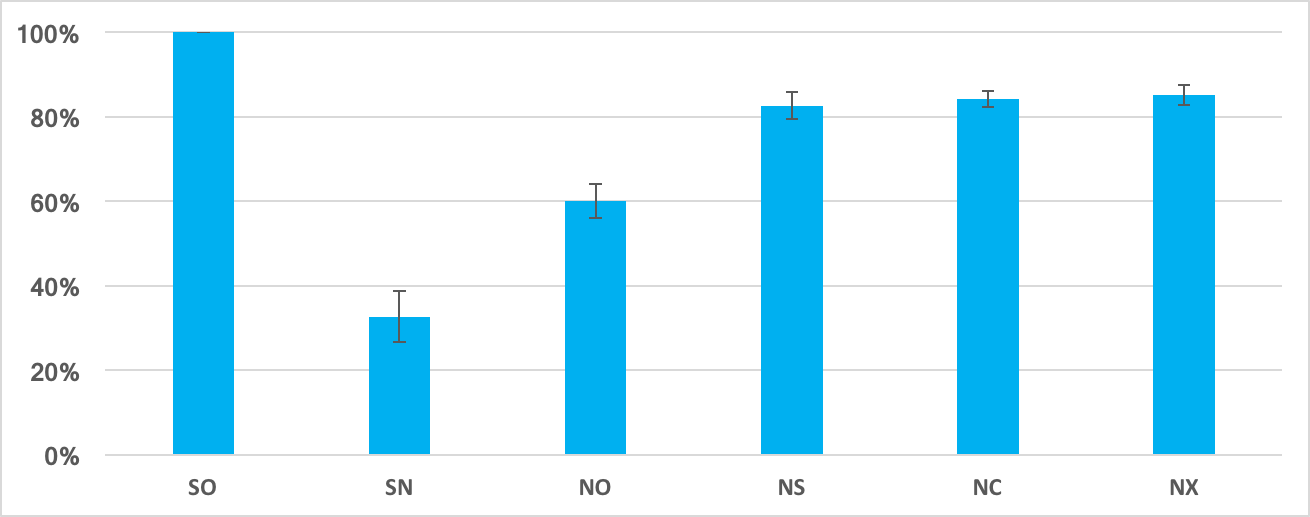
\includegraphics[max width=\textwidth]{experiment-1-results-chart}
	\caption{A comparison of the mean accuracy and 95\% confidence intervals of the models developed by the five methods.}
	\label{fig:experiment-1-results-chart}
\end{figure}

Table \ref{tab:experiment-1-results-table} and Figure \ref{fig:experiment-1-results-chart} compare the scores obtained from evaluating the models after training using the five methods. Training with symbols only (SO) produces the best model given the clear and consistent symbolic images. Training with the noisy handwritten digits only (NO) produces the worst model given the limited number of examples in the dataset. The three methods (NS, NC, NX) that developed models using noisy handwritten images as well as symbolic information show significant improvement over noisy only training. The results also show that there are no significant differences between the two methods of supplying symbols to the networks. However, the models that were trained using intermediate classification (NC and NX) have a smaller standard deviation.

\subsubsection{Discussion}

The experiments show that training a model with symbols results in a significant increase in the network accuracy over the models trained without the presence of symbols. The NC method that developed models to classify the operands as well as compute the addition did particularly well without the need for any additional inputs. The model does not accept a symbolic channel. Instead, by providing proper classification of the input operands while training, the model can be said to develop an implicit symbolic representation of the operands in the LSTM's recurrent context and transfer them from one step to the next.

The results presented in Table \ref{tab:experiment-1-results-table} and Figure \ref{fig:experiment-1-results-chart} show that there is no significant difference in the accuracy of the models trained using implicit symbols (NC) over the models trained with explicit symbols (NS). However, the experiment shows that the implicit symbol (NC) technique provides symbols to the network with the lowest predictive variance and therefore, we will use the implicit symbol technique in subsequent experiments.

Table \ref{tab:experiment-1-results-table} and Figure \ref{fig:experiment-1-results-chart} also show the results of testing the symbols only model (SO) using noisy data (SN). It is clear from the results that the network performs poorly. The model is not able to correctly map from the noisy handwritten digits to the classification labels and therefore is not able to successfully perform the addition.